% PLEASE USE THIS FILE AS A TEMPLATE
% Check file iosart2x.tex for more examples

% add. options: [seceqn,secthm,crcready]
\documentclass[aac,crcready]{iosart2x}

%\usepackage{dcolumn}

%%%%%%%%%%% Put your definitions here


%%%%%%%%%%% End of definitions

\pubyear{0000}
\volume{0}
\firstpage{1}
\lastpage{1}


\begin{document}

\begin{frontmatter}

%\pretitle{}
{\centering \title{Using linked Tableau Dashboards as Visualization Tool for MIMIC-III Data - Lessons Learned
%/A (technical) Case Report
}}
\runtitle{Tableau as Tool for MIMIC-III Data Visualization}
%\subtitle{}

% For one author:
%\author{\inits{N.}\fnms{Name1} \snm{Surname1}\ead[label=e1]{first@somewhere.com}}
%\address{Department first, \orgname{University or Company name},
%Abbreviate US states, \cny{Country}\printead[presep={\\}]{e1}}

% Two or more authors:
\author[A]{\inits{K.}\fnms{Karl} \snm{GOTTFRIED}\ead[label=e1]{k.gottfried@uke.de}%
\thanks{Corresponding Author, Karl Gottfried, Applied Medical Informatics, Hamburg, University Hospital Hamburg-Eppendorf, Martinistraße 52, 20246 Hamburg, Germany;  \printead{e1}.}},
\author[A]{\inits{S.}\fnms{Sylvia} \snm{NÜRNBERG}\ead[label=e2]{second@somewhere.com}}
and
\author[A]{\inits{F.}\fnms{Frank} \snm{ÜCKERT}\ead[label=e3]{third@somewhere.com}}
\address[A]{Applied Medical Informatics, , Germany, \orgname{University Hospital Hamburg-Eppendorf},
\cny{Germany}\printead[presep={\\}]{e1}}
\address[B]{Department first, \orgname{University or Company name},
Abbreviate US states, \cny{Country}\printead[presep={\\}]{e2,e3}}


\begin{abstract}
%The unambiguous and easy to interpret visualization of clinical patient records can help to facilitate decision making and exploration among physicians or clinicians scientists, especially with constantly growing clinical data sets. The MIMIC-III database is a freely accessible intensive care database, which documents in detail the course and treatment of more than 40,000 patients and was already used for visualization in the medical field. In the present work, we used Tableau Desktop, a commercial visual analytic software, to visualize MIMIC-III data by building so-called dashboards. This dashboard can be linked together and might be used as a potential visualization tool for clinical data. We developed three exemplary interactive dashboards to demonstrate three potential use cases which might be useful for health researchers and clinicians. One Dashboards gives the user a brief overview of the patient information stored in the data, another dashboard displays laboratory time series data for individual patients and with the third dashboard, a user will be able to select a patient cohort based on parameters like age, gender, diseases classification codes and others. Once created, dashboards can be adapted for specific questions by implementing dynamic parameters and thus reused. This approach might be useful to enable the interactive visualization and exploration of clinical data for non primarily technical users like health researchers and clinicians and also allows them to create customized dashboards for their own needs. These dashboards could be used as a starting point for further visualizations for the MIMIC-III Data and clinical data in general for instance in the context of a visualization platform for a data warehouse system. 
The unambiguous and easy to interpret visualization of clinical patient records can help to facilitate decision making and exploration among physicians or clinicians scientists, especially with constantly growing clinical data sets. The MIMIC-III database is a freely accessible intensive care database, which documents in detail the course and treatment of more than 40,000 patients and was already used for visualization in the medical field. In the present work, we used Tableau Desktop, a commercial visual analytic software, to visualize MIMIC-III data by building so-called dashboards. This dashboard can be linked together and might be used as a potential visualization tool for clinical data. We developed three exemplary interactive dashboards to demonstrate three potential use cases which might be useful for health researchers and clinicians. One Dashboards gives the user a brief overview of the patient information stored in the data, another dashboard displays laboratory time series data for individual patients and with the third dashboard, a user will be able to select a patient cohort based on parameters like age, gender, diseases classification codes and others. Once created, dashboards can be adapted for specific questions by implementing dynamic parameters and thus reused. This approach might be useful to enable the interactive visualization and exploration of clinical data for non primarily technical users like health researchers and clinicians and also allows them to create customized dashboards for their own needs. These dashboards could be used as a starting point for further visualizations for the MIMIC-III Data and clinical data in general for instance in the context of a visualization platform for a data warehouse system. 
\end{abstract}

\begin{keyword}
\kwd{Tableau}
\kwd{Data visualization}
\kwd{Patient data charts}
\end{keyword}

\end{frontmatter}

%%%%%%%%%%% The article body starts:

\section{Introduction}\label{s1}

\subsection{Background}\label{s1.1}
%Tableau is a software platform designed for visual exploration and was initially developed and used for data analysis outside of the medical field ~\cite{Tableau.2021}. Due to the continuously growing amounts of data and the desire to use this information more efficiently in a clinical and scientific context, the medical field has also become a possible application for data visualization tools like Tableau ~\cite{Ko.2017} [weitere Literatur]. 
Furthermore, Sitting et al. states that there is no standard for the visual representation of laboratory values and that every commercially available electronic health record offers its own visualization solution \cite{Sittig.2015}. According to Sitting et al. not only the simple and intuitive interpretation of laboratory values, but can also lead to misinterpretations, whereby the visualization of clinical data is also relevant for patient safety and underlines the importance of correct visualizations in clinical practice.
A clinical data source that has already been used to visualize patient data is the MIMIC-III (Medical Information Mart for Intensive Care) database, a freely accessible critical care database~\cite{Festag.2019,Lee.2016,Johnson.2020,Johnson.2016}. The third version of the MIMIC data set (MIMIC III) contains extensive clinical parameters of more than 40,000 patients who were admitted and treated in medical intensive care units of the Beth Israel Deaconess Medical Center (Boston, Massachusetts, USA) between 2001 and 2012. Collected data classes ranges from clinical measurements like nurse-verified physiological measurements, laboratory test results or administrative information like Current Procedural Terminology (CPT) codes and Diagnosis-Related Group (DRG) codes to patient characteristics like Demographic detail and dates of death or free-text interpretations of imaging studies provided by the radiology department ~\cite{Johnson.2020,Johnson.2016}. The collected data was first de-identified in accordance with Health Insurance Portability and Accountability Act standards before it was incorporated into the database. Furthermore to protect the privacy of the patients, researcher have to pass an online course and accept a data use agreement before they get access to the database ~\cite{Johnson.2020,Johnson.2016}. A demo data set with 100 patients is provided without restriction for test purposes. 
The present work uses the MIMIC Data as a clinical data set to enable specific queries with the help of Tableau, such as the visualization of time series data for certain patients or the selection of cohorts based on relevant inclusion and exclusion criteria via a visually explorable representation. In this way, for example, doctors or clinically active scientists can be presented with the relevant information through the use of dashboards and queried repeatedly with little effort.
Tableau is a software platform designed for visual exploration and was initially developed and used for data analysis outside of the medical field ~\cite{Tableau.2021}. Due to the continuously growing amounts of data and the desire to use this information more efficiently in a clinical and scientific context, the medical field has also become a possible application for data visualization tools like Tableau ~\cite{Ko.2017} [weitere Literatur]. 
A clinical data source that has already been used to visualize patient data is the MIMIC-III (Medical Information Mart for Intensive Care) database, a freely accessible critical care database~\cite{Festag.2019,Lee.2016,Johnson.2020,Johnson.2016}. The third version of the MIMIC data set (MIMIC III) contains extensive clinical parameters of more than 40,000 patients who were admitted and treated in medical intensive care units of the Beth Israel Deaconess Medical Center (Boston, Massachusetts, USA) between 2001 and 2012. Collected data classes ranges from clinical measurements like nurse-verified physiological measurements, laboratory test results or administrative information like Current Procedural Terminology (CPT) codes and Diagnosis-Related Group (DRG) codes to patient characteristics like Demographic detail and dates of death or free-text interpretations of imaging studies provided by the radiology department ~\cite{Johnson.2020,Johnson.2016}. The collected data was first de-identified in accordance with Health Insurance Portability and Accountability Act standards before it was incorporated into the database. Furthermore to protect the privacy of the patients, researcher have to pass an online course and accept a data use agreement before they get access to the database ~\cite{Johnson.2020,Johnson.2016}. A demo data set with 100 patients is provided without restriction for test purposes. 
The present work uses the MIMIC Data as a clinical data set to enable specific queries with the help of Tableau, such as the visualization of time series data for certain patients or the selection of cohorts based on relevant inclusion and exclusion criteria via a visually explorable representation. In this way, for example, doctors or clinically active scientists can be presented with the relevant information through the use of dashboards and queried repeatedly with little effort.

%%%%%%% Hier fehlt noch ein Text in etwa dieser länge
A demo data set with 100 patients is provided without restriction for test purposes. 
The present work uses the MIMIC Data as a clinical data set to enable specific queries with the help of Tableau, such as the visualization of time series data for certain patients or the selection of cohorts based on relevant inclusion and exclusion criteria via a visually explorable representation. In this way, for example, doctors or clinically active scientists can be presented with the relevant information through the use of dashboards and queried repeatedly with little effort.

In this way, for example, doctors or clinically active scientists can be presented with the relevant information through the use of dashboards and queried repeatedly with little effort.

\subsection{Objective and Requirements}\label{s1.2}
%The objective of this work is to use Tableau Desktop to create interactive and reusable visualizations for MIMIC-III data. This serves as an example use case for clinical data and evaluate the potential applicability of such visualizations as an exploration and analysis tool for a potential data warehouse system.
The created dashboards might serve as a template for visual data analysis and exploration tool so that medically trained researchers can obtain clinical information more easily.
The requirements to be met by the implemented dashboards are:
\begin{itemize}
\item A user can display the course of time-dependent variables like blood pressure for a patient or for a cohort and dynamically adjust the variable.
\item The user can select a patient cohort by dynamic filtering of variables contained in the data.
\item The dashboards should be easily expandable so that, medically trained researchers can make their own basic extensions or additions to the dashboards.
\end{itemize}
The objective of this work is to demonstrate that linked Dashboards, build with Tableau Desktop, can be used to create interactive and reusable visualizations for MIMIC-III data. We will focus on three small potential use cases which might be useful for health researchers and clinicians. This use cases are oriented on the already implemented use cases for the MIMIC III data described by the literature ~\cite{Lee.2016, Festag.2019}.
The requirements to be met by the implemented dashboards are:
\begin{description}
\item[Patient summary] A user should get an brief summary of the data that is collected for a one selected patient. The in formations shown should include all of the possible   like age, gender, diagnosis, laboratory test ect..
\item[Laboratory view] A user can check the course of time-dependent variables like blood pressure for a patient or for a cohort and dynamically adjust the variable.
\item[Cohort selection and summary] A user should be able to select a patient cohort based on all the provided data categories and check the distribution for this categories for the selected cohort.
\end{description}

The created and linked dashboards might serve as a template for visual data analysis and exploration tool so that medically trained researchers can obtain clinical information more easily.

\section{State of the art}\label{s2}
%Exploring and analyzing clinical data with visualization tools is already a known research topic~\cite{Caban.2015, Sittig.2015, UnberathPhilipp.2019, Festag.2019}. Festag et al. used KNIME analytics platform to implement a workflow for the MIMIC-III Data and the related MIMIC-III Waveform Database especially for time-series data~\cite{Festag.2019}. The user interface was implemented through so-called meta-nodes to set up the connection to both used databases in a first step~\cite{Festag.2019}. Next, a user was able to enter one or more subject IDs (representations for patients in the DB) and chooses between data sources~\cite{Festag.2019}. As the last step, the user decides which of the time series items or signals should be visualized with a line-plot ~\cite{Festag.2019}.
Another approach for MIMIC-II DB (previous version of MIMIC-III DB) was made by Lee et al. who established a data visualization tool based on web-based tools like HTML, CSS, and JavaScript libraries (jQuery and D3.js) and tools on the server side like PHP and PostgreSQL~\cite{Lee.2016}. The tool was designed to give the user a quick visualization of key aggregate statistics of the DB like sample size, distributions of clinical variables for a selected cohort. Therefore two main features were implemented, namely a explore- and a compare feature ~\cite{Lee.2016}. The Explore feature enables the user to select first a patient cohort based on variables like admission ICU service type, gender, age, and primary International Classification of Diseases 9 (ICD-9) code. In the next step further subselection was provided by the possibility to filter information like administrative information, demographic information, Interventions, lab test results, patient outcomes, vital signs and other miscellaneous variables provided by the MIMIC-II data~\cite{Lee.2016}. The Compare feature enables the user to visually compare two patient cohorts for
selected variables to be visualized~\cite{Lee.2016}. Visualization of time series data for one patient was not implemented by this project. Both attempts are promising regarding the visualization of clinical data, but setting up a hole web space with all the needed programming skills can be time-consuming and hard to maintain while handling visualizations with KNIME can be tricky and not the first choice when you think of interactive visualizations. Tableau is easy to use as a drag- and drop interface with a strong visualization capability that could meet all the requirements we identified for a tool that supports easy to use interdisciplinary data-driven research.
\subsection{Related Work}
Exploring and analyzing clinical data with visualization tools is already a known research topic~\cite{Caban.2015, Sittig.2015, UnberathPhilipp.2019, Festag.2019}. Festag et al. used KNIME analytics platform to implement a workflow for the MIMIC-III Data and the related MIMIC-III Waveform Database especially for time-series data~\cite{Festag.2019}. The user interface was implemented through so-called meta-nodes to set up the connection to both used databases in a first step~\cite{Festag.2019}. Next, a user was able to enter one or more subject IDs (representations for patients in the DB) and chooses between data sources~\cite{Festag.2019}. As the last step, the user decides which of the time series items or signals should be visualized with a line-plot ~\cite{Festag.2019}.
Another approach for MIMIC-II DB (previous version of MIMIC-III DB) was made by Lee et al. who established a data visualization tool based on web-based tools like HTML, CSS, and JavaScript libraries (jQuery and D3.js) and tools on the server side like PHP and PostgreSQL~\cite{Lee.2016}. The tool was designed to give the user a quick visualization of key aggregate statistics of the DB like sample size, distributions of clinical variables for a selected cohort. Therefore two main features were implemented, namely a Explore- and a Compare feature ~\cite{Lee.2016}. The Explore feature enables the user to select first a patient cohort based on variables like admission ICU service type, gender, age, and primary International Classification of Diseases 9 (ICD-9) code. In the next step further subselection was provided by the possibility to filter information like administrative information, demographic information, Interventions, laboratory test results, patient outcomes, vital signs and other miscellaneous variables provided by the MIMIC-II data~\cite{Lee.2016}. The Compare feature enables the user to visually compare two patient cohorts for
selected variables to be visualized~\cite{Lee.2016}. Visualization of time series data for one patient was not implemented by this project. In addition to these research projects, commercially available electronic patient records must also have a visualization component in order to display correct and easy to interpret time series variables such as laboratory values. Sitting et al. stated out for instance, that there is no standard for the visual representation of clinical data, esspecially for time series data and that every commercially available electronic health record system offers its own visualization solution \cite{Sittig.2015}. According to Sitting et al. this impede not only the simple and intuitive interpretation of laboratory values, but can also lead to misinterpretations, whereby the visualization of clinical data is also relevant for patient safety and underlines the importance of correct visualizations in clinical practice.

\subsection{Short commings}
Both attempts are promising regarding the visualization of clinical data, but setting up a hole web space with all the needed programming skills can be time-consuming and hard to maintain while handling visualizations with KNIME can be tricky and not the first choice when you think of interactive visualizations. Tableau is easy to use as a drag- and drop interface with a strong visualization capability that could meet all the requirements we identified for a tool that supports easy to use interdisciplinary data-driven research.
 
\section{Concept}\label{s3}
%For our implementation we used the commercially available software Tableau Desktop provided by Tableau\textregistered. The interaction with Tableau Desktop works by translating drag-and-drop actions into data queries via an intuitive user interface. For a first introduction of the user interface see also Ko and Chang~\cite{Ko.2017}. 
Tableau can be connected to multiple data sources like spreadsheets or text files, or for instance to a big data, relational database on a server and others. Here we used the provided 26 comma-separated values (CSV) files and build the corresponding data model based on the information about the MIMIC-III data structure provided by the PhysioNet website (https://mimic.physionet.org/). Fig.~\ref{f1} shows an overview of the used data model to interact with the data. We planed to use a patient central approach for the data model adapted to the schema provided by the SchemaSpy Analysis of MIMIC-III ~\cite{SchemaSpy.2017}. So-called worksheets are used as the basis for creating dashboards and can be individualized depending on the question.
Tableau differentiates the values present in the data according to properties such as aggregated or non-aggregated values, as well as continuous and discrete values and finally classifies them into four different categories, which can also be converted into one another. Tableau uses the following categories for measurements: a) continuous aggregate measure, b) discrete aggregate measure, c) continuous disaggregate measure, d) discrete disaggregate measure in which b) and d) are considered as dimensions by Tableau.


New data values can be added via so-called calculated fields and also displayed in the visualization. Tableau uses its own calculation syntax for the calculated fields that is reminiscent of Excel statements. Using so-called filters, data rows can be selected and also be changed dynamically using parameters. With these tools, worksheets can be specially adapted and thus used as a basis for dashboards. Dashboards are another way of interaction where individual worksheets can be linked functional together using so-called actions. Beside Tableau Desktop, Tableau offers multiple options to publish and share the created workbooks and dashboards. Tableau server for example provides browser based analytics without the need of Tableau Desktop~\cite{Tableau.20.03.2021}. 

\begin{figure}[ht]
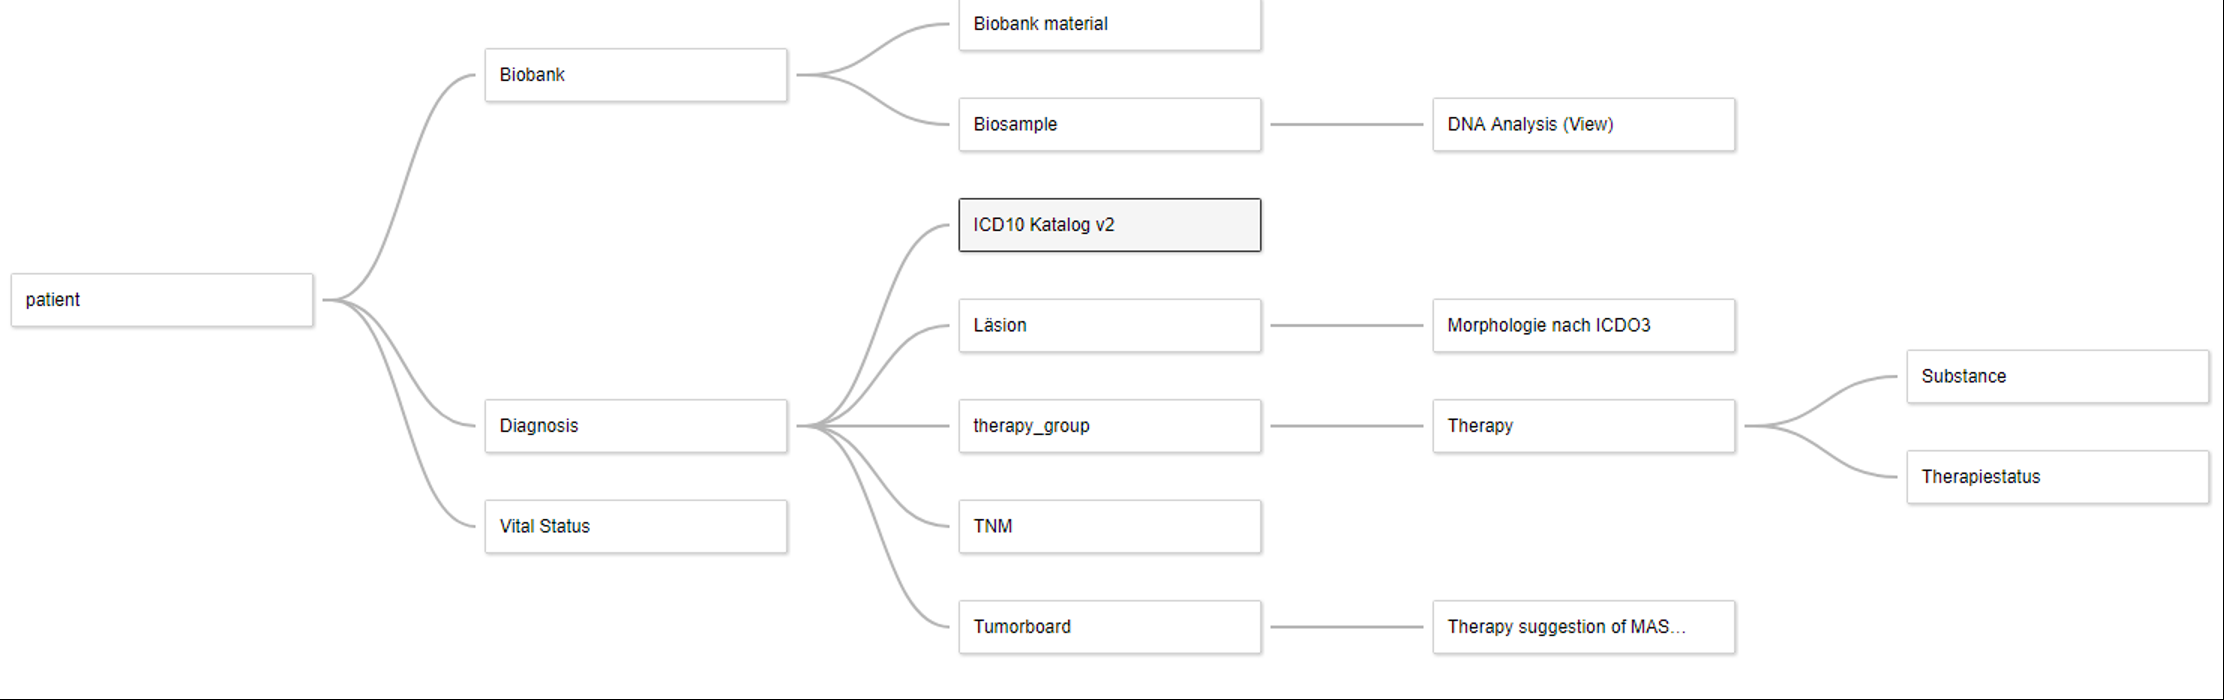
\includegraphics[width=0.7\textwidth]{images/datamodel_1.png}
\caption{Representation of the MIMIC Data Model: The squares represent CSV data tables the connections between the data tables represent the join relations used}\label{f1}
\end{figure}

\begin{table*}
\centering
\caption{Categories and their corresponding variables that the user can select to visualize}\label{t1}
\begin{tabular}{@{}ll@{}}
\hline
Category& Variables\\
\hline
Demographic information & age, ethnicity, gender, marital status, religion\\
Administrative information & admission ICU service type, admission source, admission type, number of days between ICU and hospital admissions, insurance type  \\
Patient outcomes & mortality at 28 days post-discharge from the hospital, hospital length of stay, hospital mortality, ICU mortality, ICU length of stay, 2-year survival days post-discharge from the hospital\\
Vital signs & heart rate, mean arterial blood pressure, oxygen saturation, respiratory rate, systolic blood pressure, body temperature \\
Lab test results & bicarbonate, calcium, chlorine, creatinine, glucose, hematocrit, lactate, magnesium, phosphorus, potassium, sodium, white blood cell count \\
Interventions & hemodialysis, peritoneal dialysis, total time on mechanical ventilation, vasopressor administration\\
Miscellaneous & amount of colloids administered, amount of crystalloids administered, body mass index, fluid balance, height, primary ICD-9, SOFA (sequential organ failure assessment) score, SAPS (simplified acute physiology score) I score, urine output, weight
\hline
\end{tabular}
\end{table*}
For our implementation we used the commercially available software Tableau Desktop provided by Tableau\textregistered. The interaction with Tableau Desktop works by translating drag-and-drop actions into data queries via an intuitive user interface. For a first introduction of the user interface see also Ko and Chang~\cite{Ko.2017}. 
Tableau can be connected to multiple data sources like spreadsheets or text files, or for instance to a big data, relational database on a server and others. Here we used the provided 26 comma-separated values (CSV) files and build the corresponding data model based on the information about the MIMIC-III data structure provided by the PhysioNet website (https://mimic.physionet.org/). Fig.~\ref{f1} shows an overview of the used data model to interact with the data. We planed to use a patient central approach for the data model adapted to the schema provided by the SchemaSpy Analysis of MIMIC-III ~\cite{SchemaSpy.2017}. So-called worksheets are used as the basis for creating dashboards and can be individualized depending on the question.
Tableau differentiates the values present in the data according to properties such as aggregated or non-aggregated values, as well as continuous and discrete values and finally classifies them into four different categories, which can also be converted into one another. Tableau uses the following categories for measurements: a) continuous aggregate measure, b) discrete aggregate measure, c) continuous disaggregate measure, d) discrete disaggregate measure in which b) and d) are considered as dimensions by Tableau.


New data values can be added via so-called calculated fields and also displayed in the visualization. Tableau uses its own calculation syntax for the calculated fields that is reminiscent of Excel statements. Using so-called filters, data rows can be selected and also be changed dynamically using parameters. With these tools, worksheets can be specially adapted and thus used as a basis for dashboards. Dashboards are another way of interaction where individual worksheets can be linked functional together using so-called actions. Beside Tableau Desktop, Tableau offers multiple options to publish and share the created workbooks and dashboards. Tableau server for example provides browser based analytics without the need of Tableau Desktop~\cite{Tableau.20.03.2021}. 

\begin{figure}[ht]
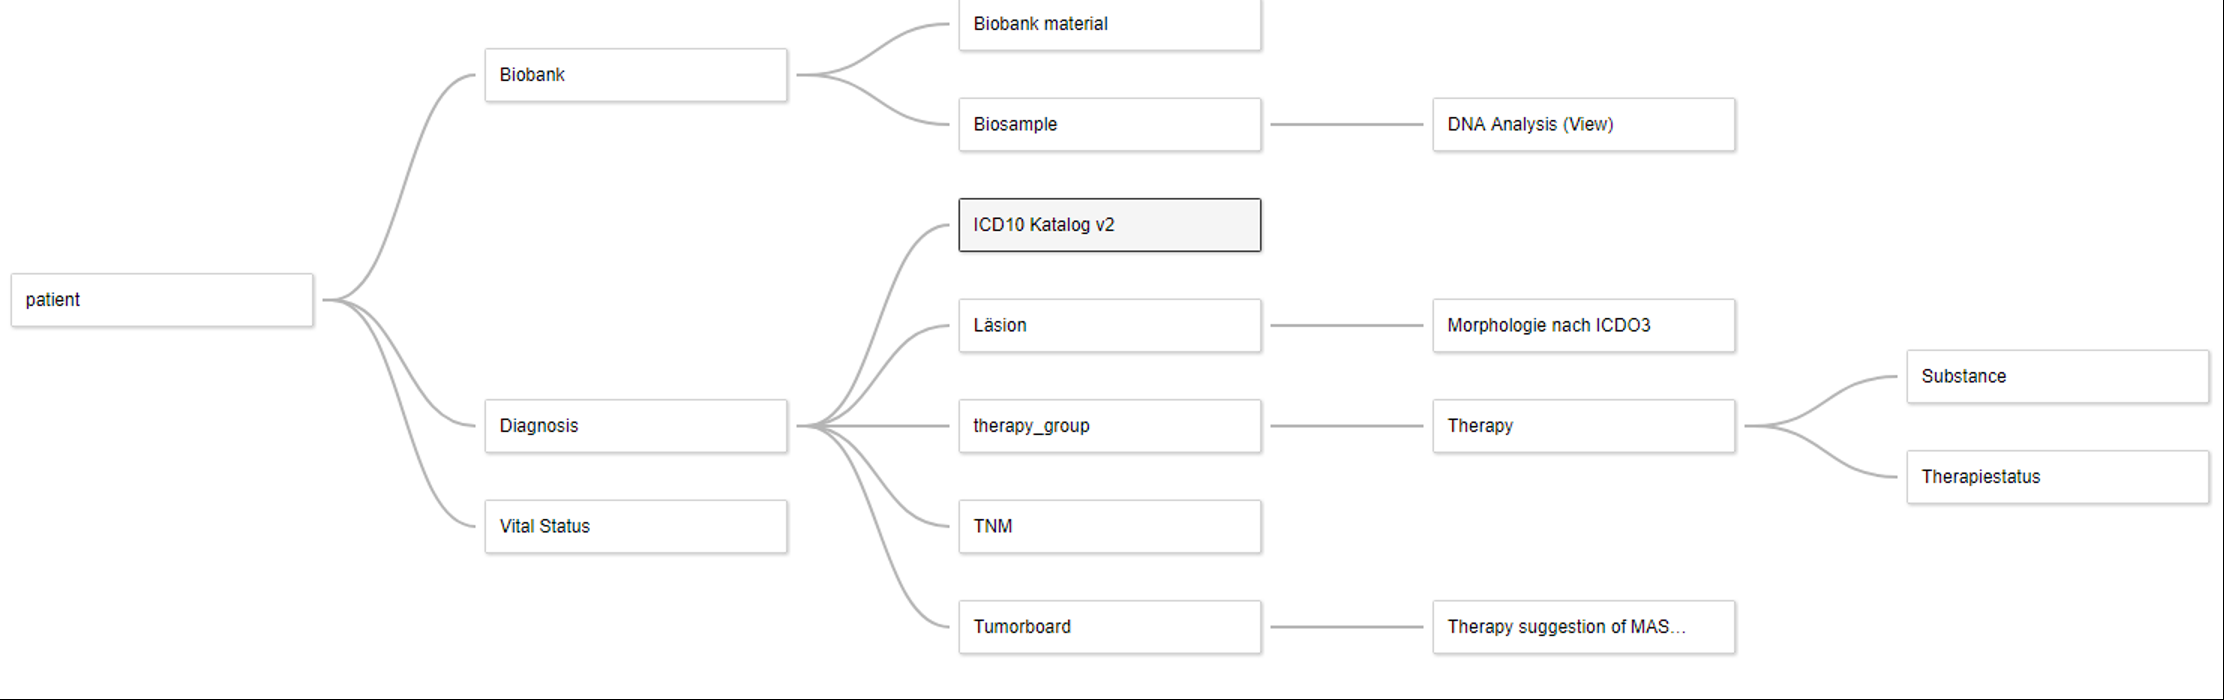
\includegraphics[width=0.7\textwidth]{images/datamodel_1.png}
\caption{Representation of the MIMIC Data Model: The squares represent CSV data tables the connections between the data tables represent the join relations used}\label{f1}
\end{figure}

\begin{table*}
\centering
\caption{Categories and their corresponding variables that the user can select to visualize}\label{t1}
\begin{tabular}{@{}ll@{}}
\hline
Category& Variables\\
\hline
Demographic information & age, ethnicity, gender, marital status, religion\\
Administrative information & admission ICU service type, admission source, admission type, number of days between ICU and hospital admissions, insurance type  \\
Patient outcomes & mortality at 28 days post-discharge from the hospital, hospital length of stay, hospital mortality, ICU mortality, ICU length of stay, 2-year survival days post-discharge from the hospital\\
Vital signs & heart rate, mean arterial blood pressure, oxygen saturation, respiratory rate, systolic blood pressure, body temperature \\
Lab test results & bicarbonate, calcium, chlorine, creatinine, glucose, hematocrit, lactate, magnesium, phosphorus, potassium, sodium, white blood cell count \\
Interventions & hemodialysis, peritoneal dialysis, total time on mechanical ventilation, vasopressor administration\\
Miscellaneous & amount of colloids administered, amount of crystalloids administered, body mass index, fluid balance, height, primary ICD-9, SOFA (sequential organ failure assessment) score, SAPS (simplified acute physiology score) I score, urine output, weight
\hline
\end{tabular}
\end{table*}

\section{Implementation}\label{s4}
%The implemented solution of the visualization tool is based on three linked tableau dashboards. Each of these dashboards consists of several workbooks, which are linked functionally by so-called actions. Each workbook of the dashboard provides subtasks for the fulfilment of the main tasks of one dashboard. Fig~\ref{fig:overviewdashboard} shows the user interface of all the three created dashboards.

\begin{figure}[ht]
   \begin{minipage}[b]{.5\linewidth}          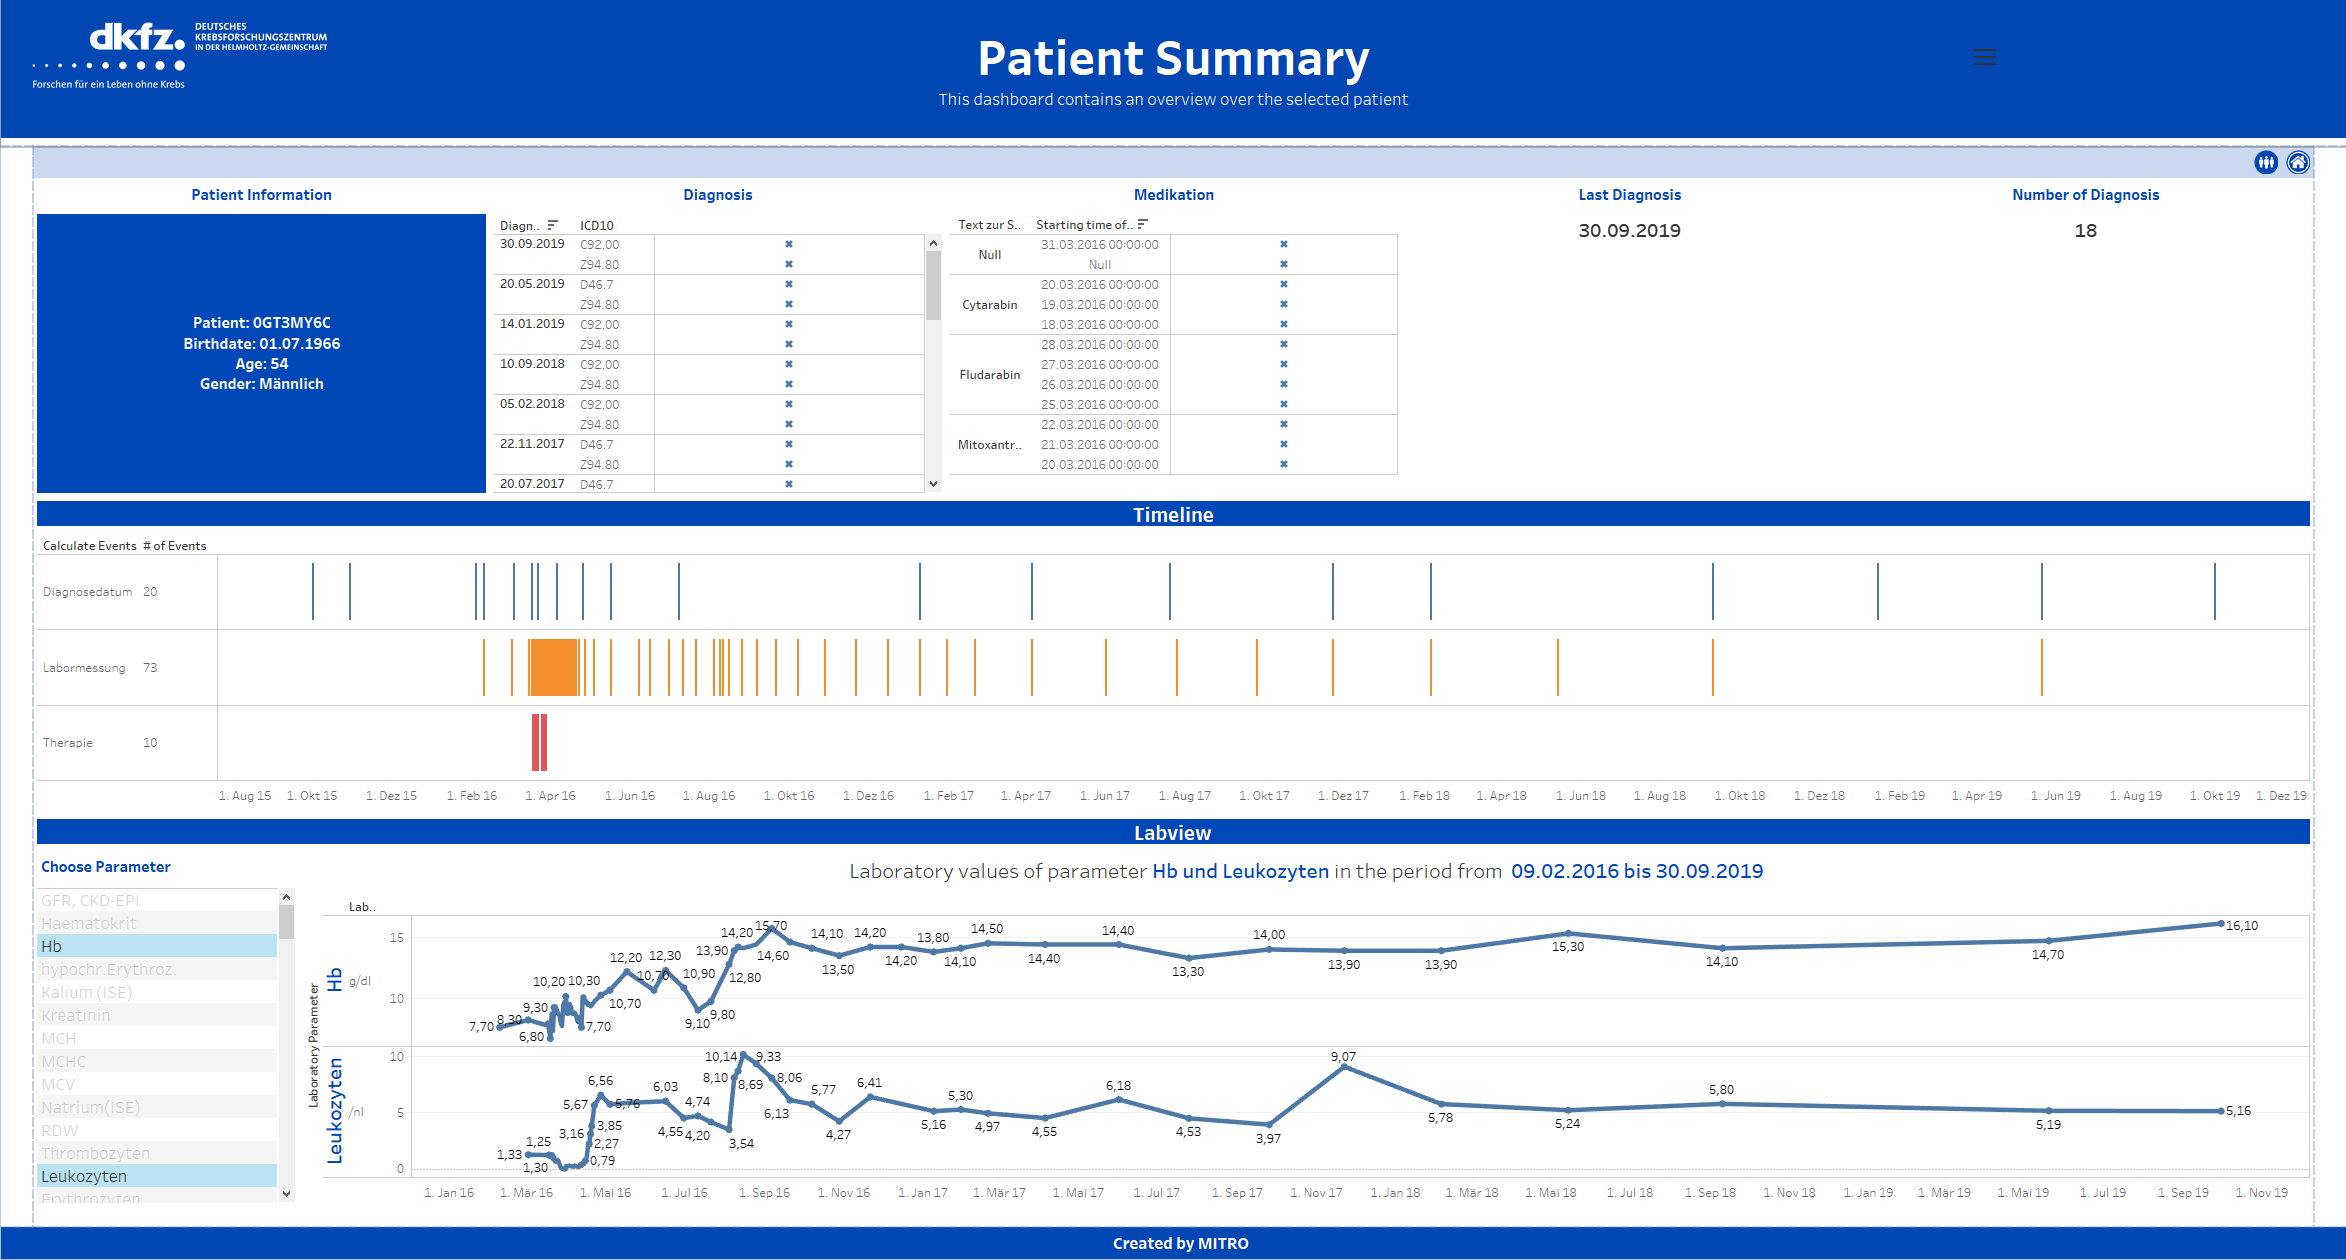
\includegraphics[width=1.05\textwidth]{images/Pat sum.png}
   \end{minipage}% 
   \hfill
   \begin{minipage}[b]{.5\linewidth} 
 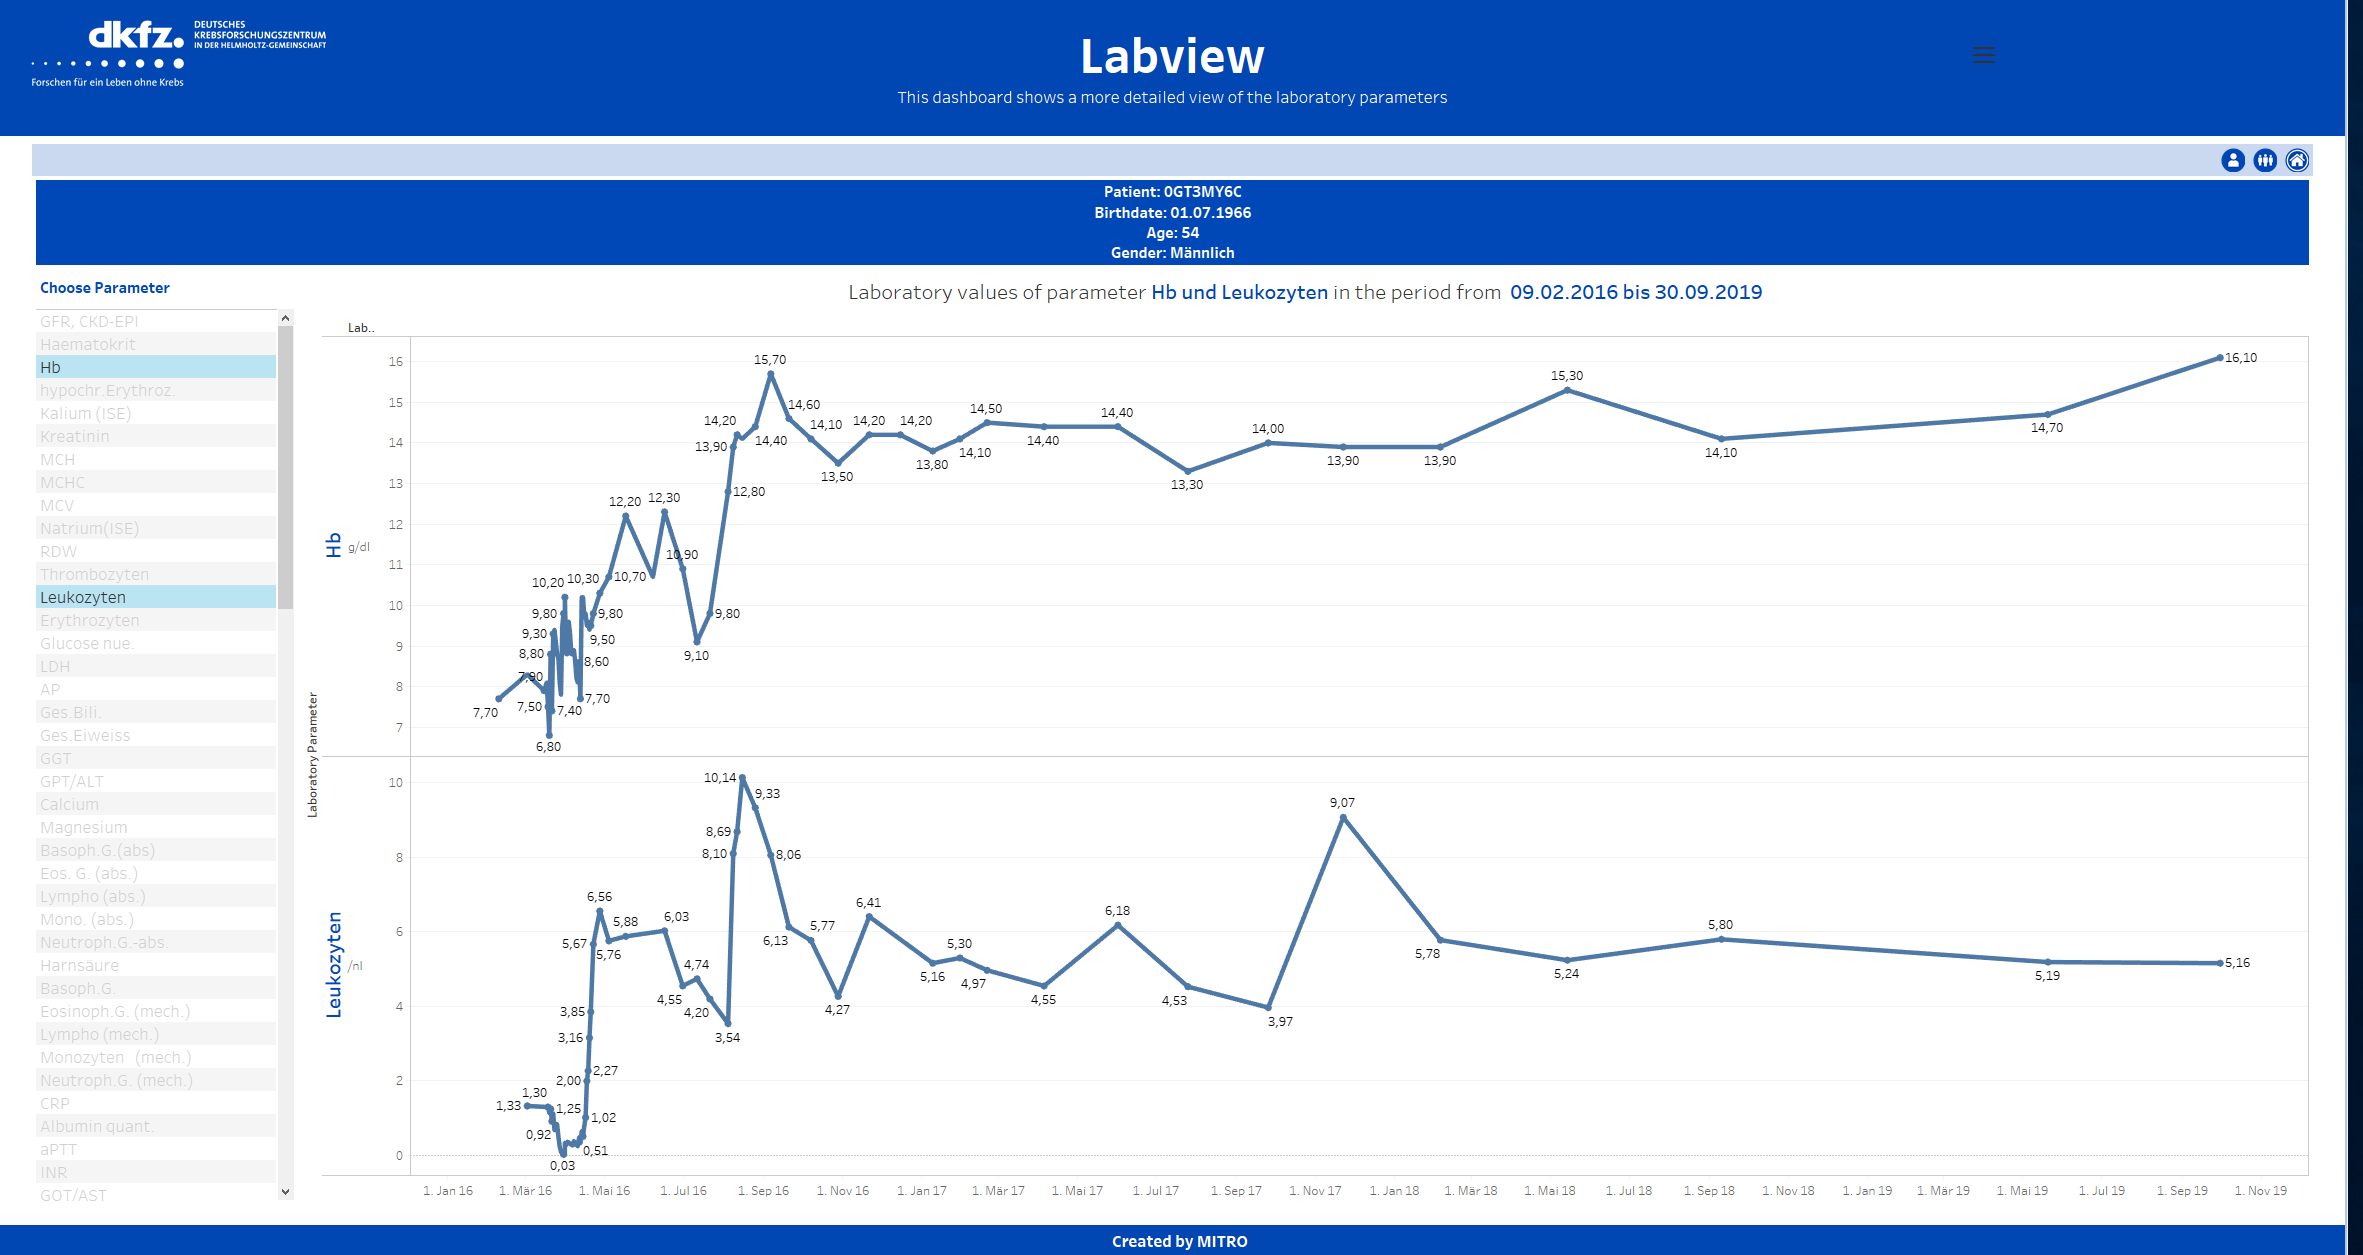
\includegraphics[width=1.05\textwidth]{images/Labview.png} 
   \end{minipage}%
   \vfill
      \begin{minipage}[b]{\linewidth}          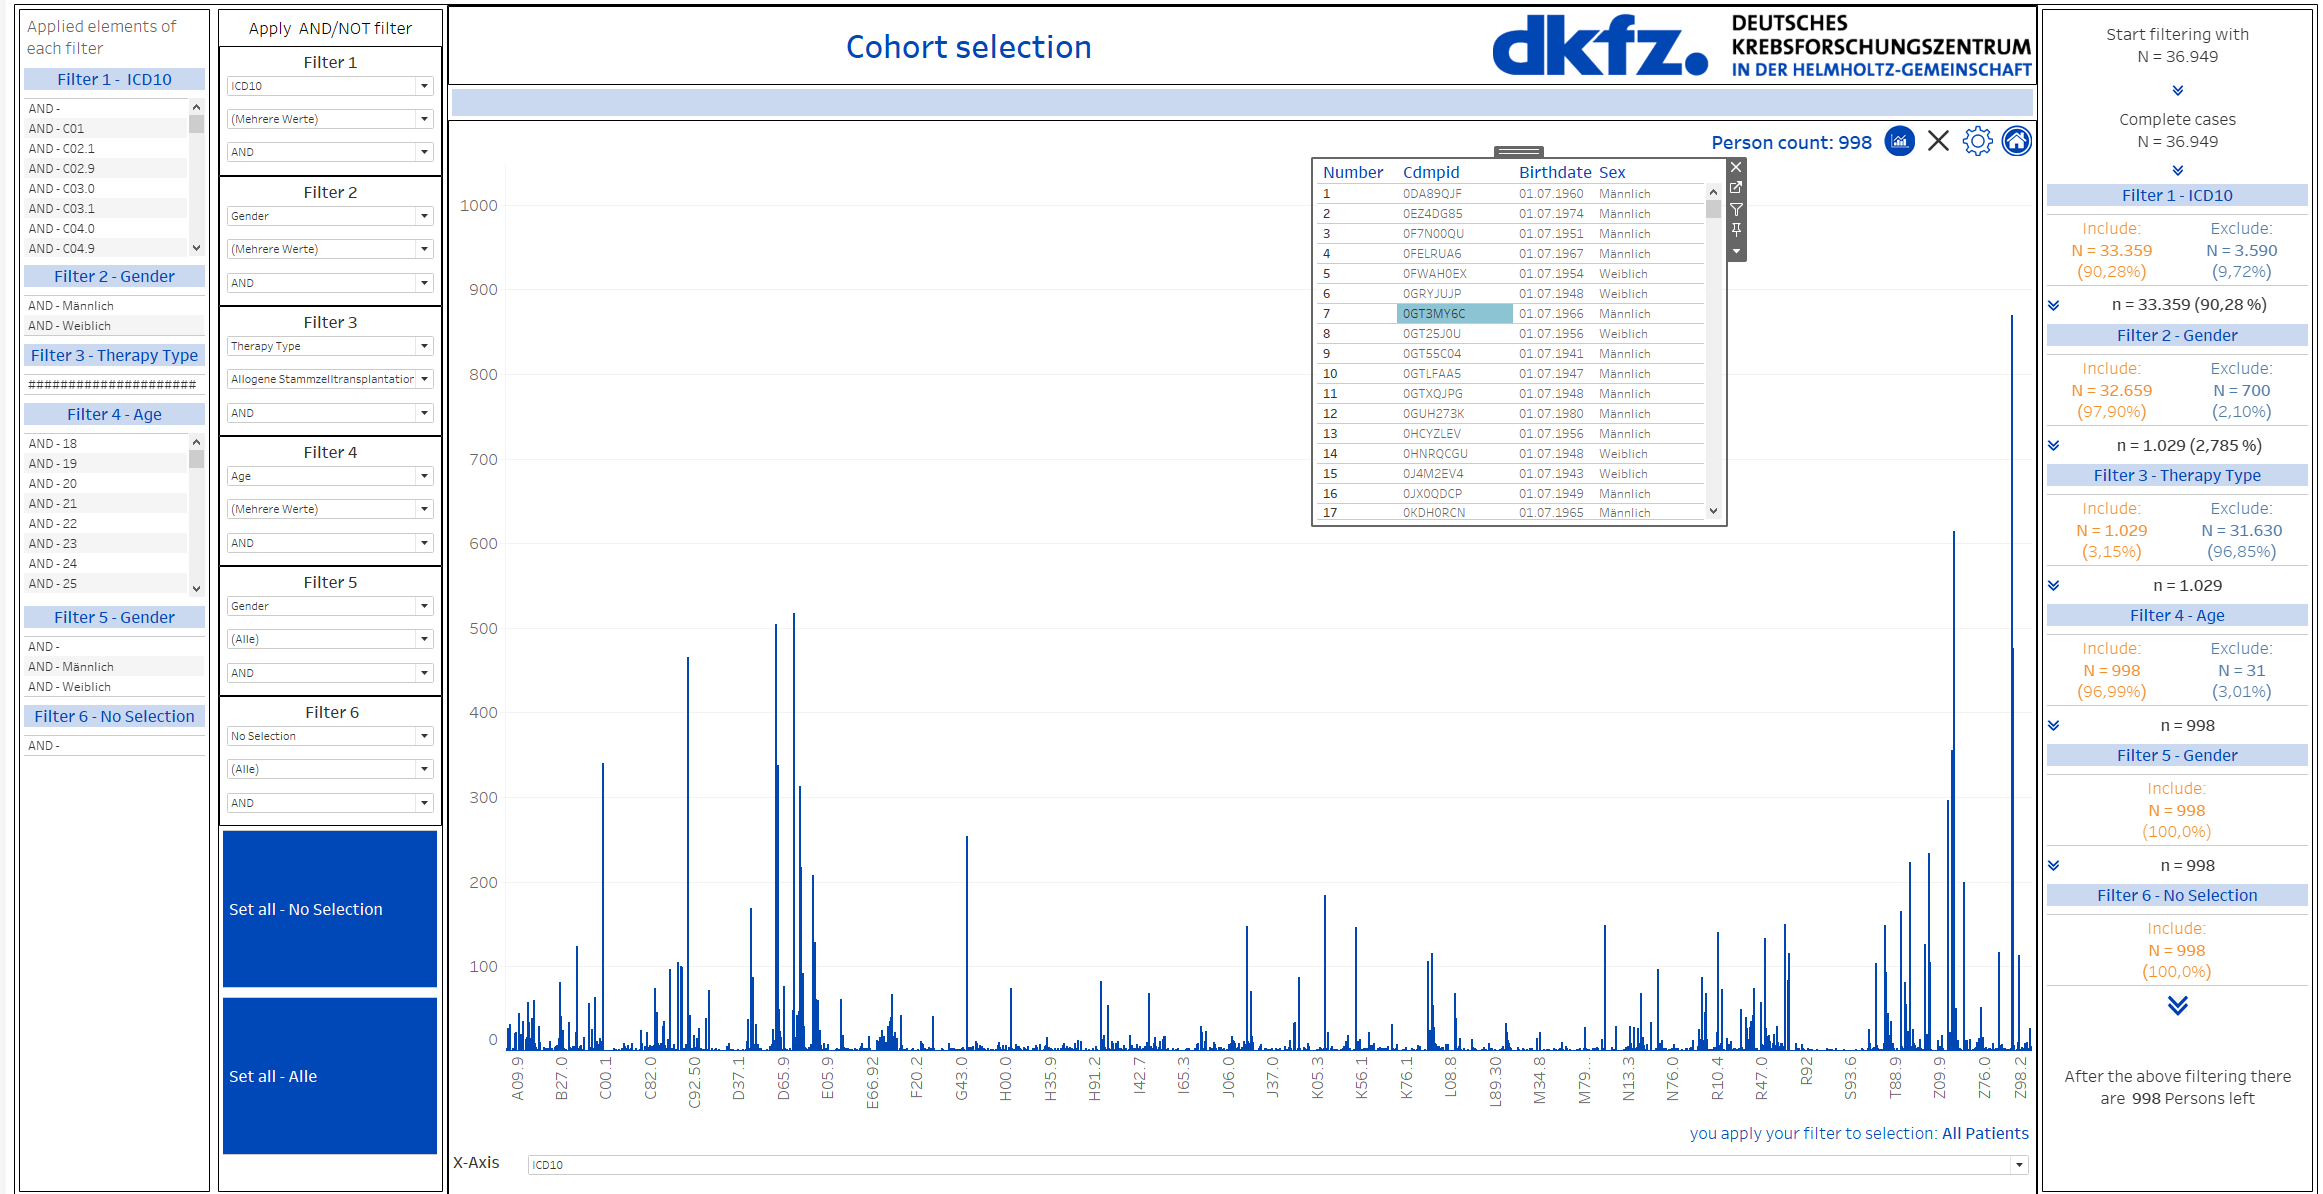
\includegraphics[width=1.05\textwidth]{images/ch sel.png}
   \end{minipage}% 
   \caption{User Interface of the three implemented dashboards}\label{fig:overviewdashboard} 
\end{figure} 

The Patient summary dashboard contains three main components. The top part contains information of the selected patient and displays variables like birthday, age, religion, eth
The implemented solution of the visualization tool is based on three linked tableau dashboards. Each of these dashboards consists of several workbooks, which are linked functionally by so-called actions. Each workbook of the dashboard provides subtasks for the fulfilment of the main tasks of one dashboard. Fig~\ref{fig:overviewdashboard} shows the user interface of all the three created dashboards.

\begin{figure}[ht]
   \begin{minipage}[b]{.5\linewidth}          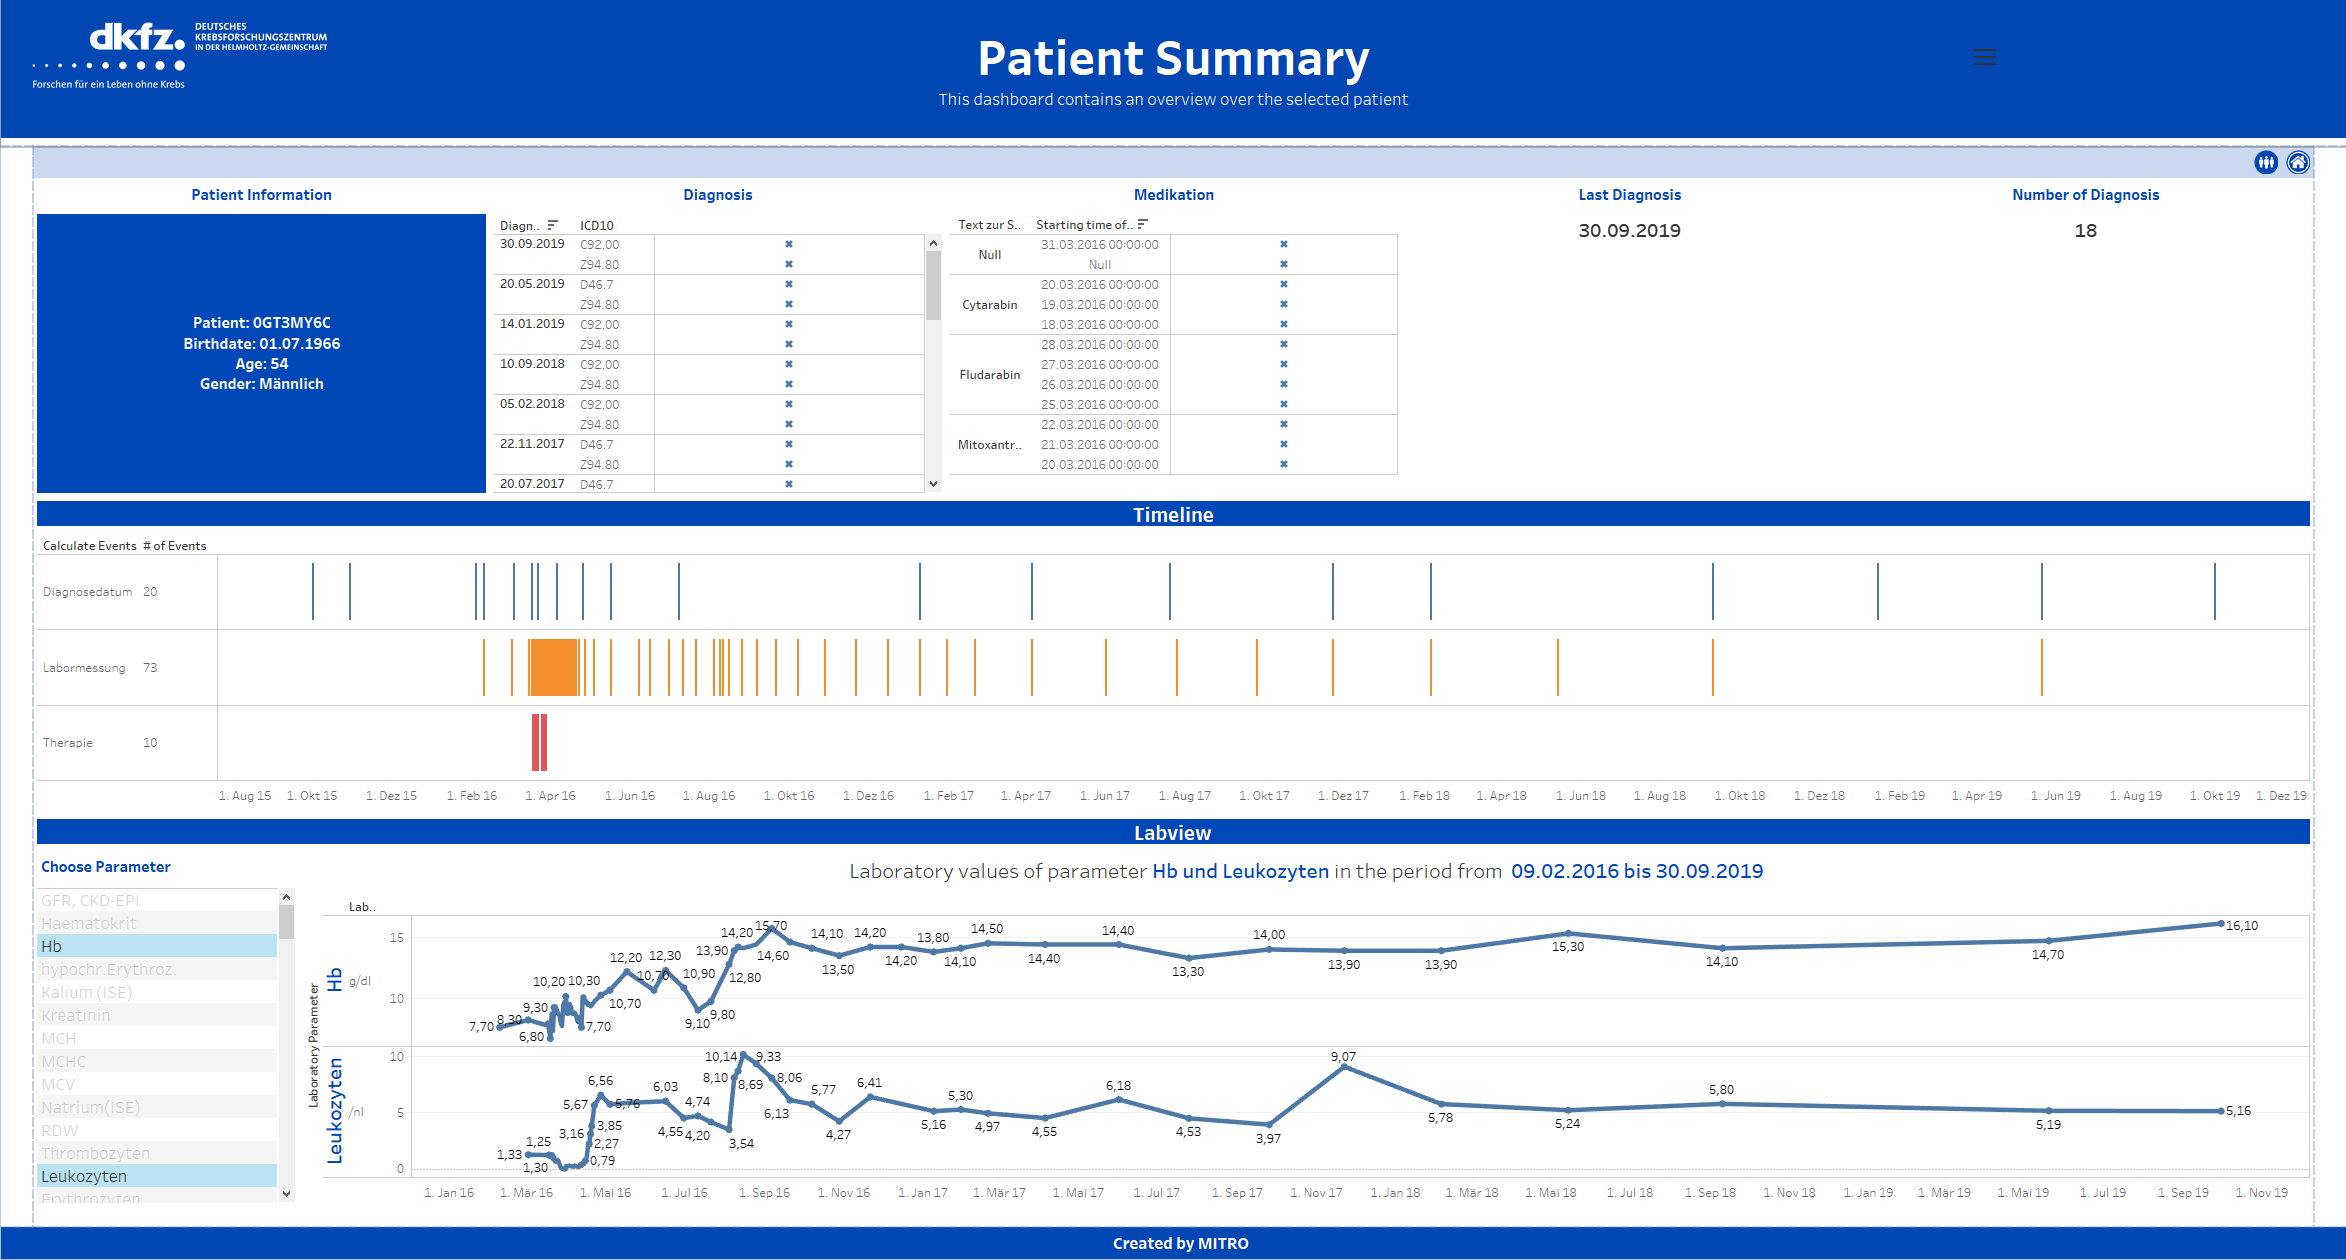
\includegraphics[width=1.05\textwidth]{images/Pat sum.png}
   \end{minipage}% 
   \hfill
   \begin{minipage}[b]{.5\linewidth} 
 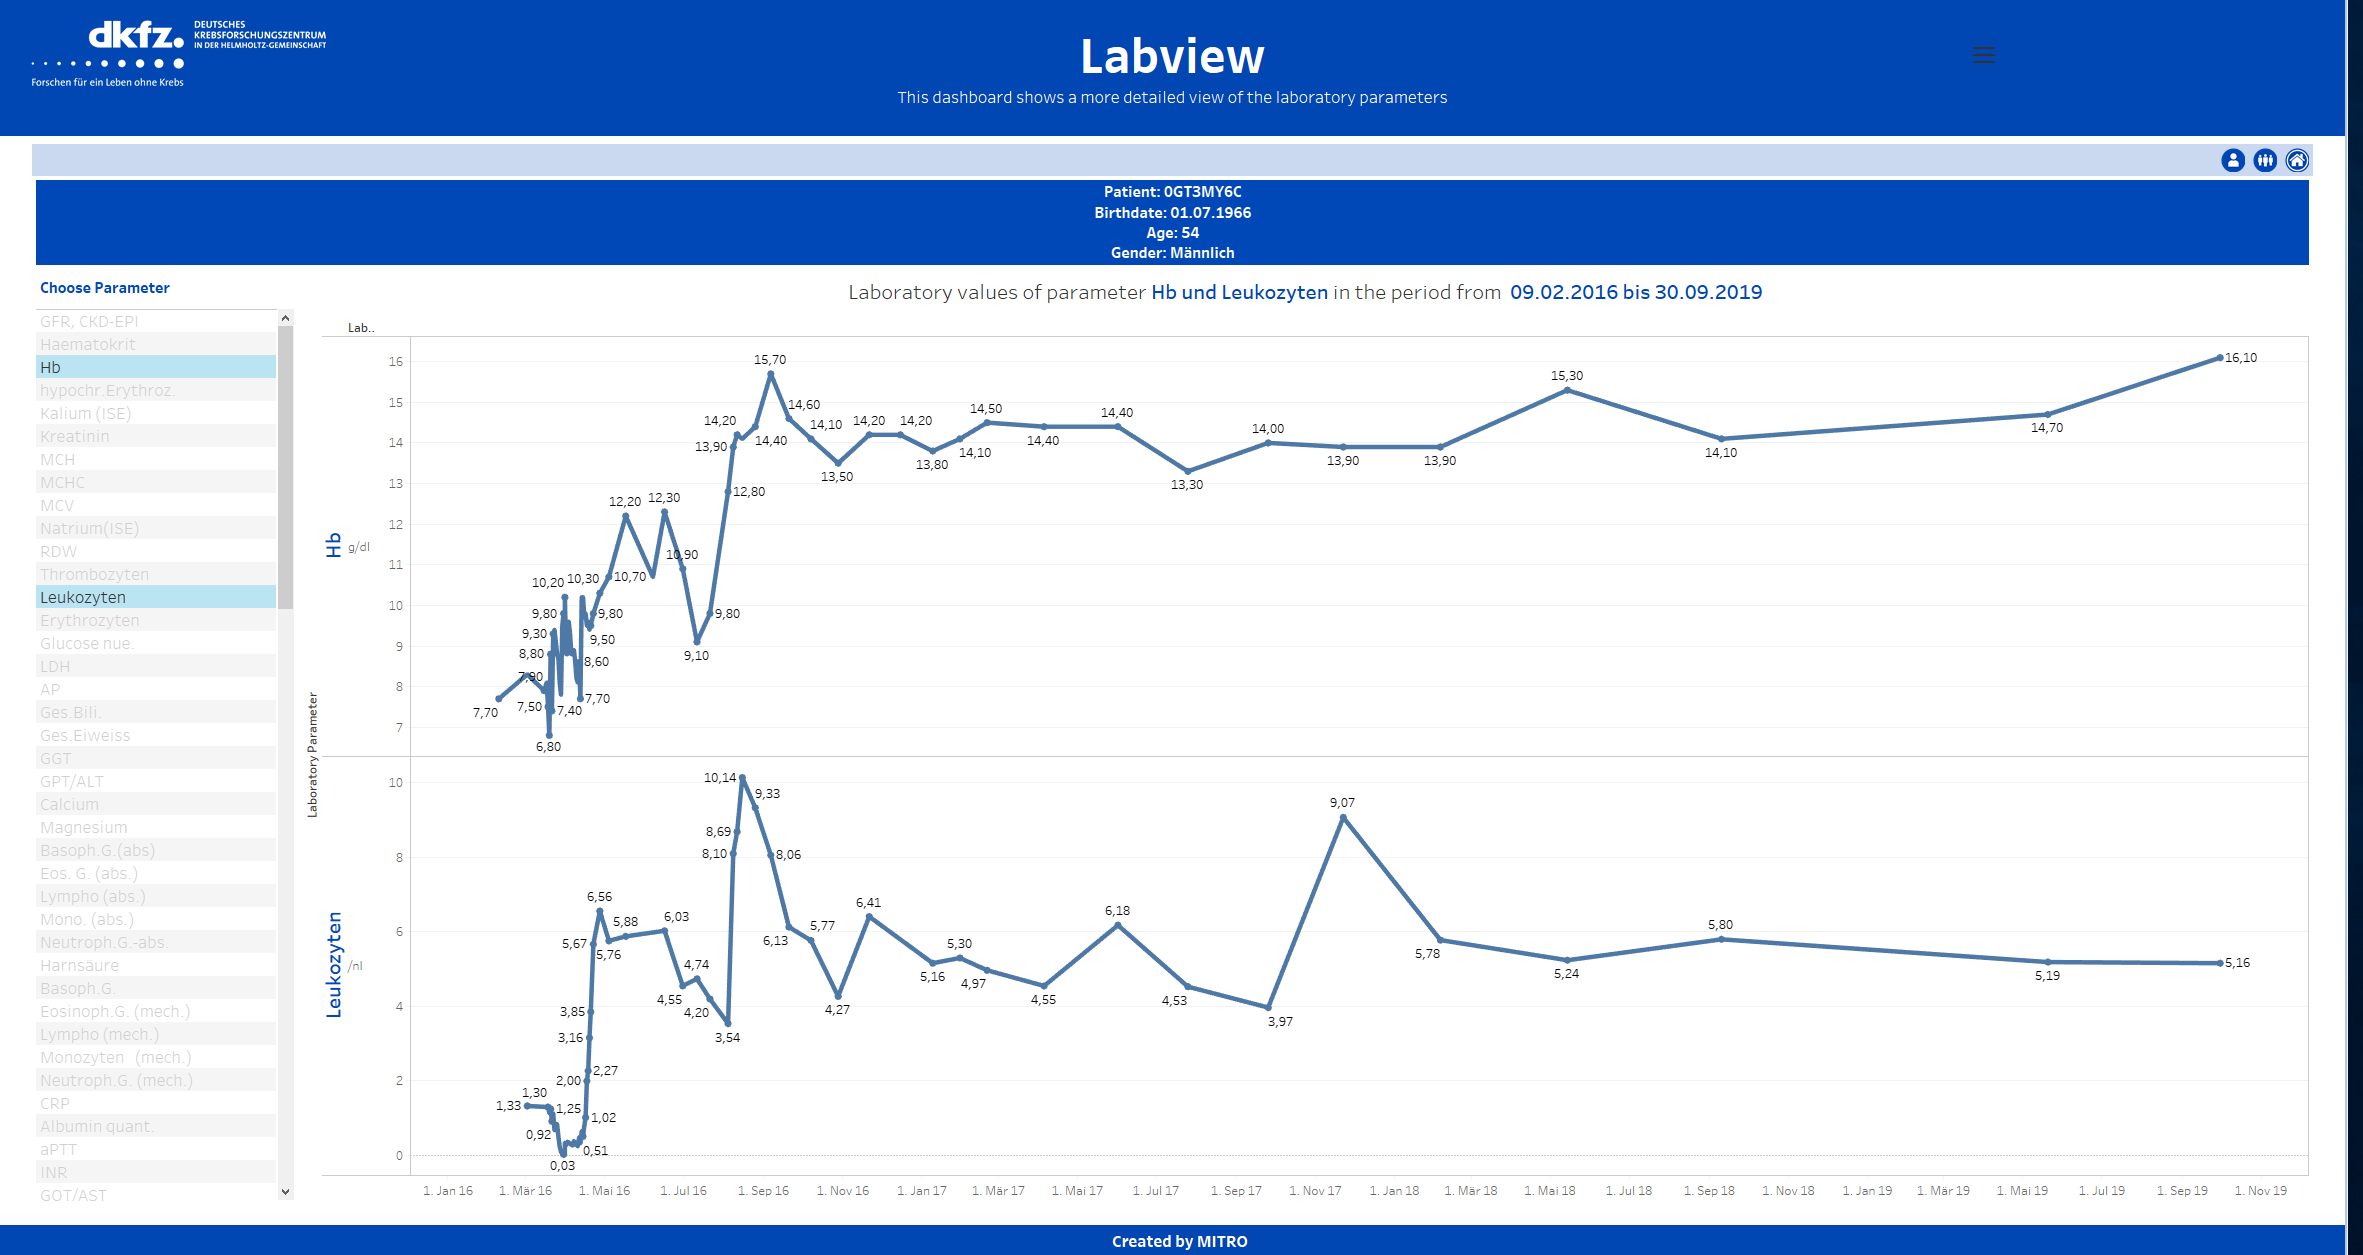
\includegraphics[width=1.05\textwidth]{images/Labview.png} 
   \end{minipage}%
   \vfill
      \begin{minipage}[b]{\linewidth}          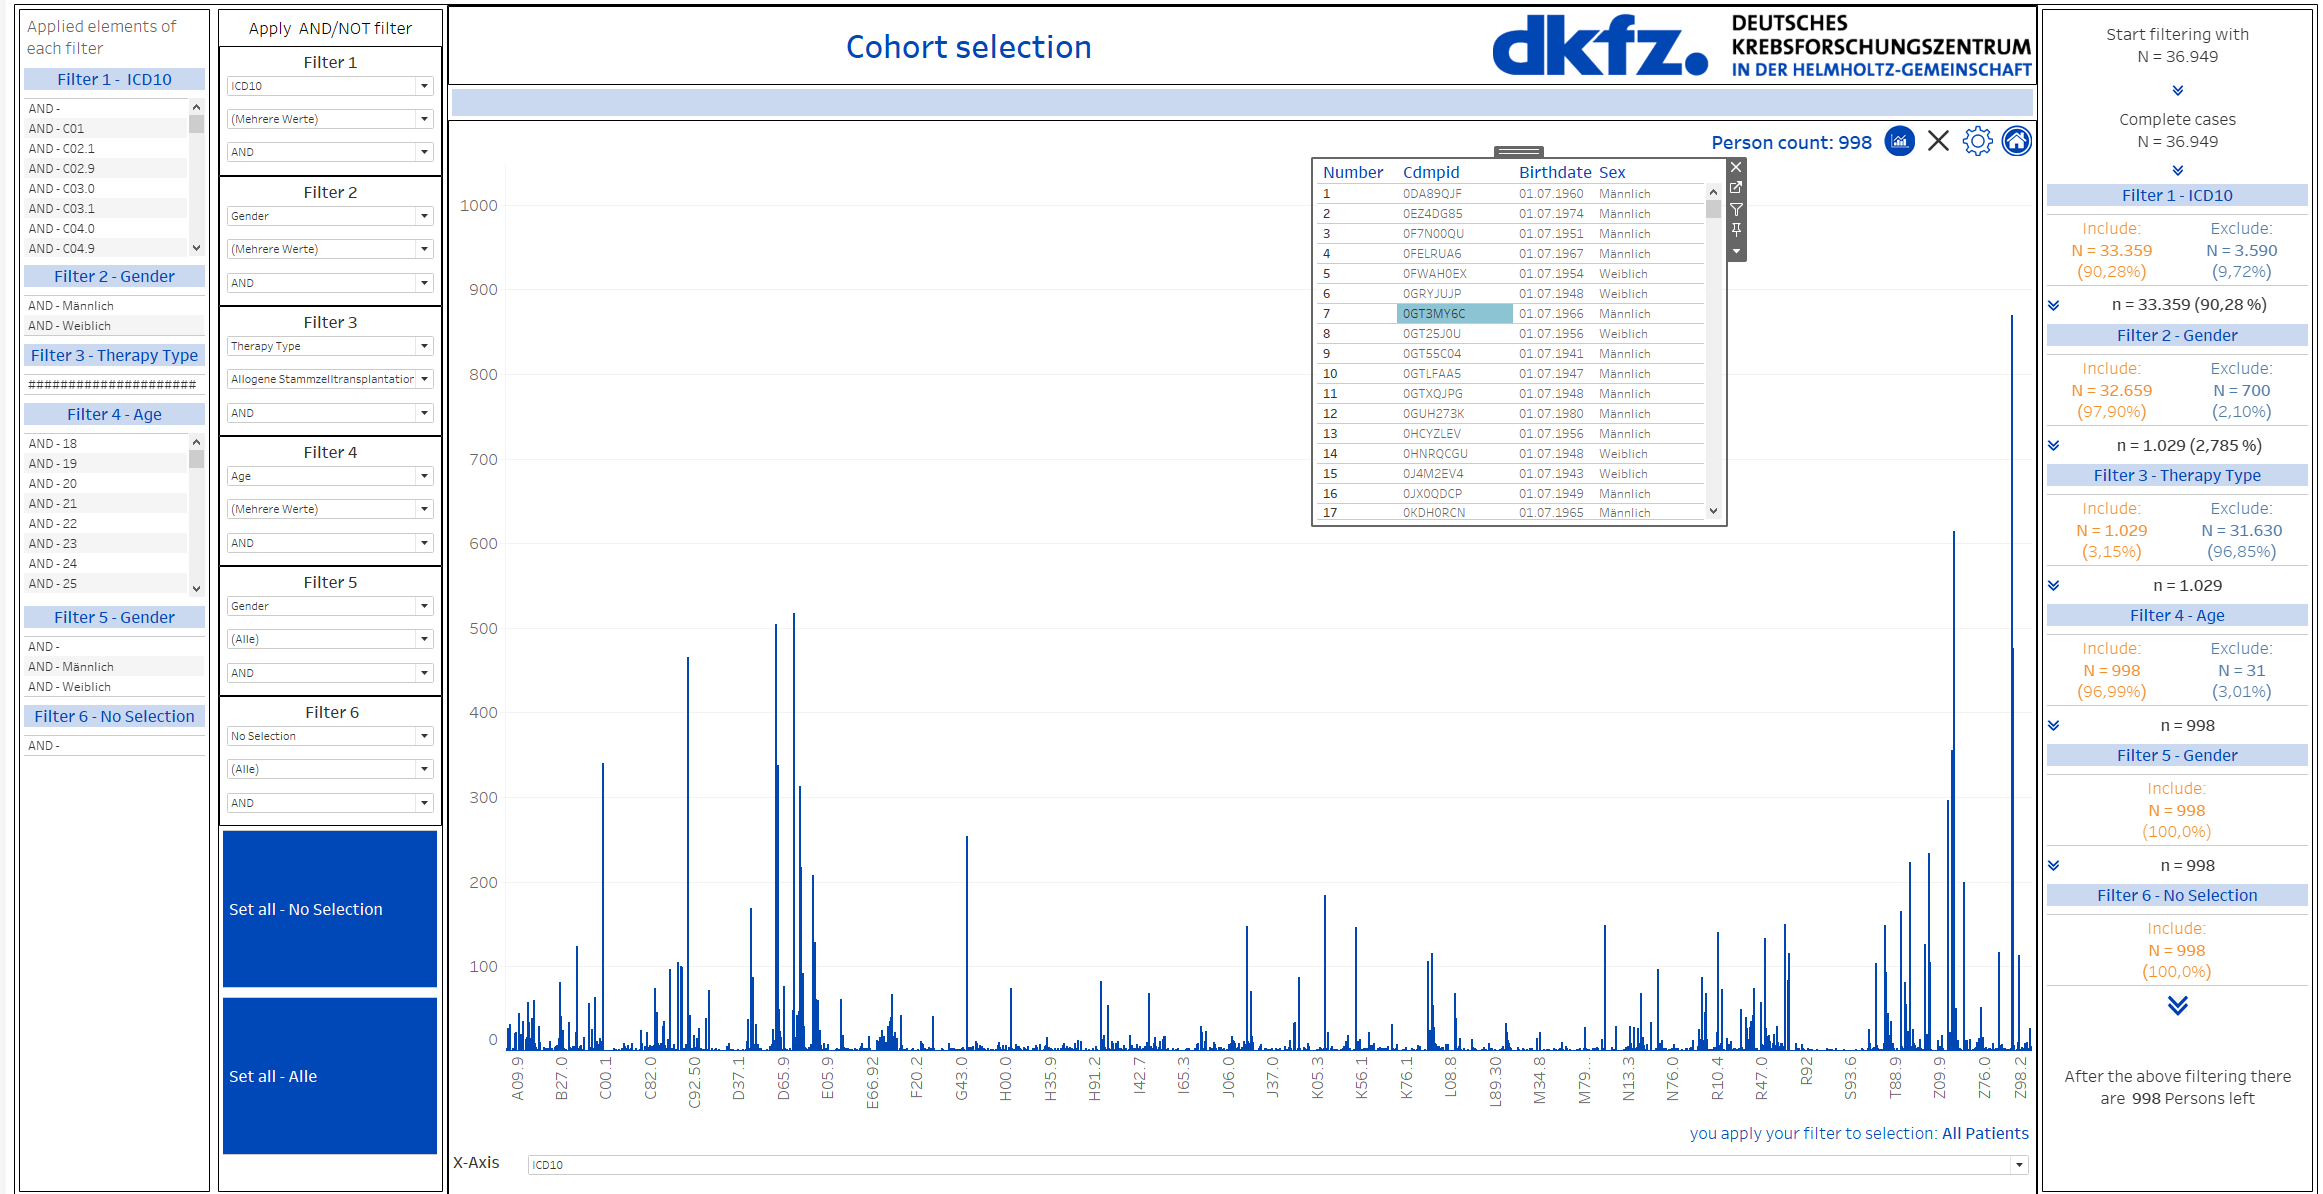
\includegraphics[width=1.05\textwidth]{images/ch sel.png}
   \end{minipage}% 
   \caption{User Interface of the three implemented dashboards}\label{fig:overviewdashboard} 
\end{figure} 

The Patient summary dashboard contains three main components. The top part contains information of the selected patient and displays variables like birthday, age, religion, eth

\section{Discussion and Outlook}\label{s5}
The dashboards created with Tableau Desktop represent a customizable and expandable presentation of clinical data. It is easy to imagine that, in addition to the area of application shown, other recurring questions can be presented, such as ...
A major limitation regarding the reusability of worksheets and dashboards with Tableau is that the visualizations or calculations depend on the correct designation and the data type used. If the name or type of a data field changes in the underlying data model over time, it may be that all the visualizations and calculations that are dependent on it have to be adapted accordingly and cannot be used. Reusability could be increased through a uniform and generally applicable data model. It is conceivable, for example, that the visualization shown is based on a general data model such as SNOMED CT instead of the MIMIC data model and can act as the basis for the data model.
Although the shown approach only displays key aggregate statistics of patients and cohort of patients it 

% mit diesem Ansatz könnte auch eine Basis von visualisierungen für klinische Daten geschaffen werden die wiederverwendet werden könnten. Wenn sich die visualisierungen auf eine einheitliche Datenbasis beziehen z.B. SNOMED CT, dann könnte man das für alle Datensysteme etablieren die dieses Model verwenden. an das Datenmodell angepasst werden und  

% Fehelende analysen bzgl. des Effekts und der Verständlichkeit der visualisierung. Wie hier dargestellt: https://pubmed.ncbi.nlm.nih.gov/31438942/

%%As there is no standard for the visualization of clinical time series data, every system uses self-designed charting tools for the display of patient data. Sittig et al. showed that a variety of widely used commercial EHRs do not optimally visualize data, which does not only hinder an easy and quick interpretation of the data, but may promote misinterpretation.
%The approach of this study combines best practices coming from literature and experts to generate a tool for unambiguous and easy to interpret time series charts. The extensible and parameterizable design of this tool allows its adaption to local preferences.

\section{Conclusion}\label{s6}
The created linked tableau dashboards represent a basic data visualization tool for MIMIC-III data and allow any researcher with data permission to perform exploration and basic analyzation on this used data set. Without any programming or database knowledge, the tool provides cohort selection options and displays patient key parameters and charts of time-series variables. The approach presented can be expanded or adapted depending on the context and thus supplement already established visualization methods for specific questions. Nonetheless, when designing and creating the data model for individual dashboards, it must also take into account that performance difficulties can arise with generic approaches, which are particularly needed in the medical field for free exploration of the data. Whether and how generic approaches can be implemented with Tableau Dashboards must be investigated in further work. An implementation of the presented dashboard with the demo data is available at the tableau public server and can be downloaded locally and be connected to the expanded data.


%\begin{figure}[t]
%\includegraphics{}
%\caption{Figure caption.}\label{f1}
%\end{figure}

%\begin{table*}
%\caption{} \label{t1}
%\begin{tabular}{lll}
%\hline
%&&\\
%&&\\
%\hline
%\end{tabular}
%\end{table*}

%%%%%%%%%%% The bibliography starts:

%%%%%%%%%%%%%%%%%%%%%%%%%%%%%%%%%%%%%%%%%%%%%%%%%%%%%%%%%%%%%
%%                  The Bibliography                       %%
%%                                                         %%
%%  ios1.bst will be used to                               %%
%%  create a .BBL file for submission.                     %%
%%                                                         %%
%%                                                         %%
%%  Note that the displayed Bibliography will not          %%
%%  necessarily be rendered by Latex exactly as specified  %%
%%  in the online Instructions for Authors.                %%
%%                                                         %%
%%%%%%%%%%%%%%%%%%%%%%%%%%%%%%%%%%%%%%%%%%%%%%%%%%%%%%%%%%%%%


\nocite{*} 
% if your bibliography is in bibtex format, use those commands:
\bibliographystyle{ios1}           % Style BST file.
\bibliography{bibliograpy_tableau.bib}        % Bibliography file (usually '*.bib')

% or include bibliography directly:
%\begin{thebibliography}{0}
%\bibitem{r1} F. Author, Information about cited object.
%
%\bibitem{r2} S. Author and T. Author, Information about cited object.
%\end{thebibliography}

\end{document}
